\documentclass[runningheads]{llncs}

\usepackage{graphicx}
\usepackage[english]{babel}
%\usepackage{cite}
\usepackage{subfig}
\usepackage{longtable}
\usepackage{natbib}
\usepackage{ulem}

\renewcommand{\bibsection}{\section{Sources}}

\begin{document}

\title{MQTT: Evaluating different types of algorithms and frameworks for achieving integrity}

\titlerunning{MQTT: Integrity}

\author{Michael Ehrlinger \and Vanessa Hermann \and Nicolas Salomon \and Martin Weinhart}

\authorrunning{M. Ehrlinger \and V. Hermann \and N. Salomon \and M. Weinhart}

\institute{University Passau, 94032 Passau, Germany}

\maketitle


\begin{abstract}
This paper depicts and evaluates different ways to ensure the integrity of a message in an MQTT environment since this is not provided by the MQTT protocol by default. 
The chosen options are Message Authentication Codes based on Hash-Functions using HMAC's, Message Authentication Codes based on Hash-Functions using Merkle Trees, Digital Signatures using Elliptic Curve Cryptography and JSON Web Signature. 
Each topic will be analysed in separate sections, to find out, which one is most suitable for achieving data integrity. 
In addition, each topic will include an example of how its presented solution has an impact on an MQTT packet. 
Apart from obvious factors like speed and security, one must not forget that MQTT can be used by all kinds of IoT-devices. 
As a result, one major aspect is also the suitability of each solution for devices with small memory and low processing speed. 
The analysis shows that the Elliptic Curve Curve25519 is most recommended to use for message integrity in an MQTT environment, due to its notable advantage over the other topics considering speed, while not performing worse concerning other relevant factors.
\newline

\end{abstract}

\keywords{MQTT \and Integrity \and JWS \and Eclliptic Curve \and Merkle Tree \and HMAC}


\newpage
\section{Indroduction}

When information is stored or transmitted using an unreliable or unsafe medium, it is essential to be able to check the integrity of the information. In an MQTT-environment, it is not uncommon to transmit data through an unreliable network, as the design considered such networks. The Message Queuing Telemetry Transport (MQTT) protocol is designed as a machine-to-machine (M2M) protocol. The protocol is like the HTTP-protocol, a Client-Server-protocol, which is used to connect Clients over a special server called a broker. The MQTT protocol distributes information using a publish/subscribe-pattern. This pattern helps cutting down the required header-information, as a subscriber sends the information to the broker, without knowing who receives the sent information. The receiver of the sent information is only known by the broker, which distributes the information to every subscriber of the topic the information belongs to. Using this pattern for a protocol brings several advantages. One advantage would be the separation of sender and receiver, so the receiver or receivers can change without interfering with the publisher, another advantage is, that the use of a broker makes it unnecessary for the publisher to include complex receiver-information with the sent packet. The missing need for receiver-information also helps by cutting down on the amount of data in the packet header. \\
In fact, the MQTT protocol is so lightweight, the header is only 2 bytes big \cite{IBM}. The downside of such a small header is that it lacks some security enhancing features, like for example some kind of integrity feature. In an IT-security aspect the word integrity can have several definitions, like “Integrity means the property that data or information have not been altered or destroyed in an unauthorized manner”\cite{INTI1} or " ”Data Integrity" means the confirmation that data which has been sent, received, or stored are complete and unchanged.” \cite{INTI2}. For achieving integrity, we look at three different algorithms and one framework in this paper. After the related work in section two, in section three we take a look at Message authentication codes using hashing, more precise HMAC, in section four we also take a look Message authentication codes using hashing, but this time using Merkle trees. In section four, we examine the use of the Edwards-curve Digital Signature Algorithm (EdDSA) to create digital signatures and in section five, we look at JSON Web Signature (JWS)-framework. After that, in section six, we evaluate the methods, we looked at in this paper, and present our recommendation.

\section{Related Work}

\subsection{Message Authentication Codes based on Hash-Functions using HMAC's}

The basic idea of HMAC’s gets defined by two standards, one provided by Request for Comments over the Internet Society (ISOC) \cite{RFC} and the other on provided by the American department of commerce as a federal information processing standards publication in the category computer security: cryptography \cite{FIBS}. Another notable standard is also provided by Request for Comments over the Internet Society (ISOC), it lists several examples for input into an HMAC generating function and the corresponding output \cite{RFC2}. The necessity to include an integrity mechanism like HMAC is also stated in the paper "Vulnerabilities and Limitations of MQTT Protocol
Used between IoT Devices" published by "Dan Dinculeană and Xiaochun Cheng" \cite{LIMI}.

\subsection{JSON Web Signature}
The JSON Web Signature (JWS) is defined an elaboratory described by the Internet Engineering Task Force Standart Track RfC 7515 \cite{rfc7515}.There are also example for the computation and validiation of a JWS with some hmacs and digital signature. Another notable Internet Engineering Task Force Standart Track is the RfC 7519 \cite{rfc7519}describing the JSON Web Token(JWT). The JSON Web Signature is a specification of the JWT.

\subsection{Digital Signatures using Elliptic Curve Cryptography}
The specific Elliptic Curve Curve25519, which this section is about, was first introduced in 2006 in the context of elliptic-curve-Diffie-Hellman functions, which Curve25519 set a new record for \cite{ECDH}. In 2012, an article in the Journal of Cryptographic Engineering depicted the speed and security of Curve25519 implemented in the context of digital signatures \cite{Curve25519}.

\subsection{Message Authentication Codes based on Hash-Functions using Merkle Trees}
The results of the work from Sebastian Rohde et al. shows „that the Merkle signature scheme provides comparable timings compared to state of the art implementations of RSA and ECDSA, while maintaining a smaller code size.“ \cite{FHB} It is also mentioned in the paper of Hongwei Li et al. That the Merkle hasht tree technique is used tu secure the communication. \cite{METR}

\section{MQTT Packet}

In this chapter a MQTT packet gets introduced, this will be used to show the impact of the presented techniques on a MQTT packet.
The used packet contains a PUBLISH-type message for the topic "/is/it/of/integrity" the contained message reads "integrity can be guaranteed, if you are able to recalculated this part:".
The content of the packet will be alter according to the newly attached content, consisting of the calculations done with the individually used techniques. \\
\newpage
The packet itself will be displayed in a hexa-decimal notation: \\

\begin{table}[]
\centering
\begin{tabular}{lllllllllllllllll}
\dashuline{45} & \dashuline{00} & \dashuline{00} & \dashuline{8d} & \dashuline{28} & \dashuline{c9} & \dashuline{40} & \dashuline{00} &  & \dashuline{80} & \dashuline{06} & \dashuline{ec} & \dashuline{47} & \dashuline{c0} & \dashuline{a8} & \dashuline{b2} & \dashuline{02} \\
\dashuline{c0} & \dashuline{a8} & \dashuline{b2} & \dashuline{06} & \dotuline{e6} & \dotuline{a4} & \dotuline{07} & \dotuline{5b} &  & \dotuline{8b} & \dotuline{bf} & \dotuline{b9} & \dotuline{65} & \dotuline{fb} & \dotuline{88} & \dotuline{a4} & \dotuline{e7} \\
\dotuline{50} & \dotuline{18} & \dotuline{01} & \dotuline{00} & \dotuline{05} & \dotuline{b0} & \dotuline{00} & \dotuline{00} &  & 30 & \uwave{5c} & 00 & 13 & 2f & 69 & 73 & 2f \\
69 & 74 & 2f & 6f & 66 & 2f & 69 & 6e &  & 74 & 65 & 67 & 72 & 69 & 74 & 79 & 69 \\
6e & 74 & 65 & 67 & 72 & 69 & 74 & 79 &  & 20 & 63 & 61 & 6e & 20 & 62 & 65 & 20 \\
67 & 75 & 61 & 72 & 61 & 6e & 74 & 65 &  & 65 & 64 & 2c & 20 & 69 & 66 & 20 & 79 \\
6f & 75 & 20 & 61 & 72 & 65 & 20 & 61 &  & 62 & 6c & 65 & 20 & 74 & 6f & 20 & 72 \\
65 & 63 & 61 & 6c & 63 & 75 & 6c & 61 &  & 74 & 65 & 64 & 20 & 74 & 68 & 69 & 73 \\
20 & 70 & 61 & 72 & 74 & 3a &    &    &  &    &    &    &    &    &    &    &    \\  
\end{tabular}
\caption{MQTT-packet with the according markers}
\label{tab:my-table}
\end{table}
A MQTT-packet does not only consist of MQTT specific data, it also consists of other protocols, which are needed for submitting the packet.
This additional information is made up from control information needed for the transport of the packet. The part underlined with a dashed line marks the Internet Protocol (IP), the underlining with a dotted line marks the Transmission Control Protocol (TCP).
The main parts of the here visible packet, will remain unchanged, even when more information is added later down the line, there is only one byte, which indicates the remaining length of the MQTT packet, that will be changed according to the attached piece of information, the current value is correct for a remaining length of 92 bytes and is marked by a waved line in the packet.
\section{Message Authentication Codes based on Hash-Functions using HMAC's}

In this section, we will look at and evaluate the use of Hash-functions on the message authentication code sent with messages in an MQTT environment. \\
%Message authentication code%
A message authentication code (MAC) gets send with the message from the sender to the receiver so that the receiver can authenticate the content of the received message. \\
%Why use mac with hash in the first hand?%
Hash-Functions find wide use in constructing a MAC. The reasons for this are a faster execution time than for symmetric block chippers, an essential feature in low power IoT-devices. A second reason is good availability for library code providing suitable hashing algorithms, so used functions are known to work as intended. 
%Def hash-function%
\subsection{Definition of HMAC}
Before going more into detail, I want to clarify what is meant by a hash function. ''We assume H to be a cryptographic hash function where data is hashed by iterating a basic compression function on blocks of data. We denote by B the byte-length of such blocks, and by L the byte-length of hash outputs. The authentication key K can be of any length up to B, the block length of the hash function. Applications that use keys longer than B bytes will first hash the key using H and then use the resultant L byte string as the actual key to HMAC. In any case, the minimal recommended length for K is L bytes. [\dots] We define two fixed and different strings ipad and opad as follows (the ’i’ and ’o’ are mnemonics for inner and outer)
\begin{center}
ipad = the byte 0x36 repeated B times \\
opad = the byte 0x5C repeated B times.
\end{center}
To compute HMAC over the data ‘text’ we perform 
\begin{center}
H(K XOR opad, H(K XOR ipad, text))''
\end{center}
\cite{RFC}.  \\
% This definition can be used only for hash-functions, which require a secret key to compute a hash value. The use of a key is necessary, because without a secret key, everyone, who knows the hash function, used to compute the MAC, could compute a valid MAC according to the actually invalid message and therefore making the use of a MAC irrelevant. \\

%Using underlying hash functions%
When using a hash function to compute a MAC, the underlying hash-function is used as a black-box \cite{KHF}, so that the function itself could be swapped out without affecting the rest of the code. The reasons for keeping the use of the actual hash-function so flexible are, ease of maintainability, ease of testing and ease of upgradeability. The first two are connected because its recommended to choose a hash function, where the code is open-source, which gives the piece of code support, so possible threats are detected and bugs get fixed sooner. The ease of upgradeability comes through the encapsulation of the code, done to achieve the black-box effect, which supports the already mentioned swapping of hash-functions.
The most commonly used hash-functions to generate a MAC are either MD5 or SHA-1 (\cite{CRY-MD5}, \cite{NPC}), for all of these are implementations available and they are widely adopted. Of course, when using any kind of function to achieve more security, it is essential to know about possible flaws of the used function. 
%Security consideration of underlying hash functions%
\subsection{Advantages}
\subsubsection{Security of underlying hash function}
Both MD5 and SHA-1 are cryptographic hash function, so their basic mechanism is to compress an input I to an output O of a specific length L. L is only influenced by the function itself, not by the input. In case of MD5, this output O is 128 bits or 16 bytes \cite{BAV} long when using SHA-1 the output is 160 bits or 20 Bytes \cite{BAV} long. Any hash-function used in a security-sensitive area should be considered secure, that a hash-function is considered secure, it needs to have preimage resistance, second-preimage resistance and collision resistance. The relation between these three resistances is the following, ''collision resistance implies second preimage resistance and second preimage resistance implies preimage resistance'' \cite{SPR-res}. Through this implication chain, it can be concluded, that when collision resistance gets refuted, this also falls back to second preimage resistance and preimage resistance. Unfortunately, both hash-functions, MD5(\cite{COL1}, \cite{COL2}) and SHA-1(\cite{COL3}, \cite{COL4}), are known to have collisions. At first glance, these found collisions seem to make MD5 as well as SHA-1 a bad choice for generating HAMCs, as HMAC can only be defined as secure, when the underlying hash-function was weakly collision resistant, ''The results are for NMAC but can be lifted to HMAC.
 %It is shown in [3]\% 
[\dots] that NMAC is a secure PRF if (1) the underlying compression function h is a secure PRF, and also (2) that the hash function H is weakly collision resistant (WCR).'' \cite{HMAC-SEC1}(The here mentioned NMAC stands for Nested MAC, which is a way to construct MAC's using pseudorandom-functions \cite{NMAC}). This means, if there are collisions for the underlying hash-function, the resulting HMACs cannot be considered secure, but this definition changed, it was proven, ''that NMAC is a PRF under the sole assumption that the underlying compression function h is itself a PRF. In other words, the additional assumption that the hash function is WCR is dropped. (And, in particular, as long as h is a PRF, the conclusion is true even if H is not WCR, let alone CR.)'' \cite{HMAC-SEC1}. This last statement speaks only about NMAC, but as it was stated in a prior statement, ''The results are for NMAC but can be lifted to HMAC.'' \cite{HMAC-SEC1}. So even though both MD5 and SHA-1 can no longer be considered collision resistant, as shown above, this does not affect their use as an underlying hash function for computing HMAC's.
%Angriffsarten für hmac% 
\subsubsection{Not much useable attack vectors}
Even now, when collisions in the underlying hash-functions are no longer compromising the security of HMACs, there are other possible attacks, which could compromise the security and so also the use of HMAC. The attack vectors know to HMAC are called distinguishing attack and forgery attack. The distinguishing attacks divide in distinguishing-H and distinguishing-R attacks, the difference between the two is, ''Distinguishing-R attack means distinguishing a MAC from a random function, and distinguishing-H attack detects an instantiated MAC (by an underlying hash function or block cipher) from a MAC with a random function.''\cite{ATT1}. A distinguishing-R attack can be made using the so-called birthday paradox. It requires about 2\textsuperscript{(n$/$2)} messages (n is the length of the output of the hash function) and works with a probability of 63\%\cite{ATT1}. The most famous example of the birthday paradox is that in a room with a minimum of 23 people, there is a chance from up to 86\% that two people share the same birthday not considering their year of birth. This probability seems to be very high for the number of needed messages, but even after a successful distinguish-R attack there is a single random HMAC compromised, the to compromise HMAC cannot be chosen beforehand, so the actual probability of distinguishing a useful message can be considered low, the actual probability depends on the used underlying hash-function. The probability that a distinguish-H attack is successful is about 2\textsuperscript{-n}\cite{ATT1} (n is the length of the output of the hash function). This probability again depends on the length of the output of the underlying hash function. The probability of a successful distinguish-H attack needs to be so low as it is, because here a preselected message gets distinguished, so the use of a single successful attack is much higher. 
%Key length/Hashlength%
\subsubsection{Manageable Keylength and Hashlength}
When computing an HMAC value, the definition states, that there is a specific key used, which also serves as a shared secret between sender and receiver. This key should be chosen randomly. The suggestion is that a key should be as long as a block of the underlying hash function, it is stated that such a block is 64 byte for both MD5 and SHA1 \cite{RFC}. Longer keys do not increase the strength directly but can help when the random-function used for key generation is weak. Shorter keys are also possible, but the minimum size is the length of the output of the hash-function \cite{RFC}. There is no clear guideline for key replacement given, as there are no known practical attacks, which could exploit such a key \cite{RFC}. \\
As already stated, the length of the output depends on the hash function itself, MD5 produces a 128 bit or 16 bytes hash and SHA-1 produces a 160 bit or 20 bytes hash. \\
%Truncated output%
''A well-known practice with message authentication codes is to truncate the output of the MAC and output only part of the bits'' \cite{RFC}. The basic idea of truncation is to shorten the output produced by the hash function. This brings both advantages and disadvantages. An advantage would be given less information to a possible attacker. A disadvantage would be that there are lesser bits that need prediction when attacking. Cutting away more than n/2 (n is the length of the output of the hash function)is not recommended, because otherwise, it would match a boundary for the birthday-attack as mentioned above. 
%Computing time comparison(material)%
\subsubsection{Quick Computing time}
HMAC’s are used as a security enhancing feature, but next to the security features speed plays an essential role because the best security is beginning to seem useless when securing a packet is by far the most complicated thing in the whole chain. The speed is given in Throughput, so how much data can be processed per time unit when using MD5 the throughput is 756,0 MB/S \cite{MAX}, this comes down to 12096 message blocks per second or 0,08ms (=milliseconds) per block. When using SHA-1, the throughput goes up to 1024,0 MB/s \cite{MAX}, this comes down to 16384 message blocks per second or 0,06ms.

\subsection{Disadvantages}
The use of HMAC as a measurment for integrity does not come with any directly attached disadvantages. In the form of a too high computation time, a to large overhead or a too large key to store on the device. \\
Despite this missing directly attached disadvantages, there is a disadvantage,, in the form of missing self implementation.
For the use of HMAC, a hash function and an xor function is necessary, if the developer does not implement these for himself or even check for the correctness of the used open source functions, he will be vulnerable. This vulnerability is present, but it will be very small in most cases, because the more people working on and using this pieces of code, the better the maintancen and correctness will be(as already stated in section4.1). 

\subsection{Impact on MQTT packet}
%key: e9r3rZrvAqEMkAFRpXP9m8pNAXYAQmT4TcmAdHusePWQBspX98bMxHfkp0bHcNWG
%encoded: 4c 1a 7b 15 1e 24 50 c8 cf cf 93 b0 30 cd c7 16 71 dc 49 13
%Hexcode for length: 01110000
After learning the theoretical aspects of HMAC,the next step is looking at the real life impacts on a MQTT packet.
As mentioned in the chapter "Manageable Keylength and Hashlength" a key used with the HMAC algorithm should be as long as a block length of the used hash function. The hash function used in this example will be SHA-1, a block of SHA-1 is 64 bytes long, so the used key will be just as long. \\ The used key will be "e9r3rZrvAqEMkAFRpXP9m8pNAXYAQmT4TcmAdHuse\\PWQBspX98bMxHfkp0bHcNWG" \\
When using this key to encode the message of the basis paket "integrity can be guaranteed, if you are able to recalculate this part:" the result looks like this "4c 1a 7b 15 1e 24 50 c8 cf cf 93 b0 30 cd c7 16 71 dc 49 13", when already written in hexa-decimal encoding. When the HMAC part gets attached to the packet, the length of the packet gets extended, so the corresponding field need to be changed as well, to enable a correct reading, the length grows from 133 to 153 bytes.\\
After attaching the HMAC part and changing the length field the basis packet now looks like this:
\begin{table}[]
\centering
\begin{tabular}{lllllllllllllllll}
45 & 00 & 00 & 8d & 28 & c9 & 40 & 00 &  & 80 & 06 & ec & 47 & c0 & a8 & b2 & 02 \\
c0 & a8 & b2 & 06 & e6 & a4 & 07 & 5b &  & 8b & bf & b9 & 65 & fb & 88 & a4 & e7 \\
50 & 18 & 01 & 00 & 05 & b0 & 00 & 00 &  & 30 & 6f & 00 & 13 & 2f & 69 & 73 & 2f \\
69 & 74 & 2f & 6f & 66 & 2f & 69 & 6e &  & 74 & 65 & 67 & 72 & 69 & 74 & 79 & 69 \\
6e & 74 & 65 & 67 & 72 & 69 & 74 & 79 &  & 20 & 63 & 61 & 6e & 20 & 62 & 65 & 20 \\
67 & 75 & 61 & 72 & 61 & 6e & 74 & 65 &  & 65 & 64 & 2c & 20 & 69 & 66 & 20 & 79 \\
6f & 75 & 20 & 61 & 72 & 65 & 20 & 61 &  & 62 & 6c & 65 & 20 & 74 & 6f & 20 & 72 \\
65 & 63 & 61 & 6c & 63 & 75 & 6c & 61 &  & 74 & 65 & 20 & 74 & 68 & 69 & 73 & 20 \\
70 & 61 & 72 & 74 & 3a & 4c & 1a & 7b &  & 15 & 1e & 24 & 50 & c8 & cf & cf & 93 \\
b0 & 30 & cd & c7 & 16 & 71 & dc & 49 &  & 13 &    &    &    &    &    &    &    \\  
\end{tabular}
\caption{Basis packet with attached HMAC and modded length field}
\label{tab:my-table}
\end{table}



\section{Message Authentication Codes based on Hash-Functions using Merkle Trees}

To guarantee the integrity of transfered data, there is the possibility to use Merkle Trees on Message Authentication Codes (MAC) alongside hash-functions like it is described in chapter three in this paper. Merkle Trees are hash trees named after the scientist Ralph Merkle „where the value associated with a node is a one-way function of the nodes’s children. For many applications, one wishes to output a sequence of consecutive leaves (or leaf pre-images), along with their “authentication paths” – the latter consists of the interior nodes that constitute the siblings on the path from the leaf to the root. Given an authentication path and a leaf, one can verify the correctness of the latter with respect to the publicly known root value.“ \cite{MT} 

\begin{figure}
\centering
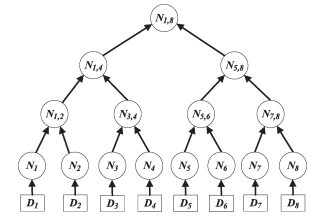
\includegraphics[width=6cm]{Pages/Merkle/merkleTree.png}
\caption{Merkle Tree Structure \cite{METR}}
\end{figure}

In figure 1 - Merkle Tree Structure the data (d) is shown with the letter „D“ and the nodes are represented with the letter N. The data itself is not considered part of the Merkle Tree. The Nodes h(D\textsubscript{i})(i = 1,..., 8) are the hashed values of the data and this is where the Merkle Tree starts. Nodes in the same row are considered as siblings and the nodes above are their parents, which values are deviated from their children. Nodes without children are called leaf nodes. This hash tree is also called binary tree because every parent has two children. Binary trees have a height H with $ 2^{H} $ leaves, and $  2^{H} $ - 1 nodes. \cite{MT} 
For example the hash value of node N1,2 is h1,2 = h(h1|h1), and the hashed value of the node N1,8 is h1,8 = h(h1,4|h5,8). \cite{METR} The node on the top is also called root node and contains the final hash value. Every child node can be affirmed with the root node and its authentication path information (API). For example, the integrity of node N1 can be verified from the server that stores the hashed value h1,8 as: „N1 sends D1 and the corresponding API = h2, h3,4, h5,8 to the server. Then, the server can check the authenticity of node N1 by first computing h1, h1,2 = h(h1|h2), h1,4 = h(h1,2|h3,4), h1,8 = h(h1,4|h5,8). And then, the server checks whether the computed h1,8 is the same as the existing h1,8“. \cite{METR} N1 will only be accepted by the server, if both values are the same. So that means that you can look at a part of a file to check if this is correct without having the entire thing available.

\subsection{Outcome and hashing}
To hash the data you have to choose a function that is able to do this. One choice would be, for example, SHA-1 with a length of 128 bit.
„The value of a leaf, in turn, is a one-way function of some leaf preimage. For small trees these pre-images may be simply stored; alternatively for larger trees, the leaves may be calculated with a keyed pseudorandom generator.“ \cite{MT} Because the hash functions are the only thing that have to be computed, the computation time, regarding the verification, is quite low. \cite{METR} In a Merkle Tree structure it is desired to generate an output sequence fore every leaf that has two components; the leaf pre-image, and the authentication path (Fig 2 - Authentication Path) \cite{MT}

\begin{figure}
\centering
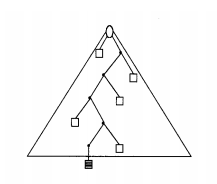
\includegraphics[width=5cm]{Pages/Merkle/API.png}
\caption{Authentication Path [JLMS03]}
\end{figure}

The circle in Fig. 2 represents the root node; the grey square is the leaf’s pre-image, and the white squares biuld the authentication path of the grey square.

\subsection{Security and speed}
„Since software implementations of hash functions are much more efficient than software implementations of finite field arithmetic, the Merkle signature scheme (MSS) is a good candidate for implementations on small microprocessors without cryptographic coprocessors“. \cite{FHB} Like mentioned before, the hash function is the only thing that has to be computed and so it is inportant to choose a propper one regarding to it’s cryptographic properties because MSS relies only to it. So that is on the one hand a big benefit and on the other hand a disadvantage if it is found insecure. But if the hash function appears to be insecure, it can be easily replaced with a secure one to make the MSS save again. Also the signature generation is faster than RSA and comparable to ECDSA. Further performance improvements are reached by utilizing a symmetric crypto engine such as an AES hardware acceleration. \cite{FHB}  "The total space
required is bounded by $ 1.5 log^2 $  N/loglog N hash values, and the worstcase computational effort is 2 log N/loglog N hash function evaluations
per output." \cite{MT}

\subsection{Impact on MQTT packet}
Signing a packet with a digital signature will have an impact to the packet itself. An example of how a MQTT packet looks like after its integrity is guaranteed using a Merkle Tree is shown in table 3 - MQTT paket with attached MAC using a Merkle Tree. In this example SHA-1 is the used hash function. If we use the Merkle Tree method on the sentence that was mentioned before which is "integrity can be guaranteed, if you are able to recalculate this part:", the result is: f7 87 ec 5e be 3e 5c 53 2c 3c 7b d2 04 94 c8 21 44 39 4b 18. This has to be attached to the MQTT paket to ensure its security and therefore the the length increases from 133 to 153 bytes.

\begin{table}[]
\centering
\begin{tabular}{lllllllllllllllll}
45 & 00 & 00 & 8d & 28 & c9 & 40 & 00 &  & 80 & 06 & ec & 47 & c0 & a8 & b2 & 02 \\
c0 & a8 & b2 & 06 & e6 & a4 & 07 & 5b &  & 8b & bf & b9 & 65 & fb & 88 & a4 & e7 \\
50 & 18 & 01 & 00 & 05 & b0 & 00 & 00 &  & 30 & 5b & 00 & 13 & 2f & 69 & 73 & 2f \\
69 & 74 & 2f & 6f & 66 & 2f & 69 & 6e &  & 74 & 65 & 67 & 72 & 69 & 74 & 79 & 69 \\
6e & 74 & 65 & 67 & 72 & 69 & 74 & 79 &  & 20 & 63 & 61 & 6e & 20 & 62 & 65 & 20 \\
67 & 75 & 61 & 72 & 61 & 6e & 74 & 65 &  & 65 & 64 & 2c & 20 & 69 & 66 & 20 & 79 \\
6f & 75 & 20 & 61 & 72 & 65 & 20 & 61 &  & 62 & 6c & 65 & 20 & 74 & 6f & 20 & 72 \\
65 & 63 & 61 & 6c & 63 & 75 & 6c & 61 &  & 74 & 65 & 20 & 74 & 68 & 69 & 73 & 20 \\
70 & 61 & 72 & 74 & 3a & f7 & 87 & ec &  & 5e & be & 3e & 5c & 53 & 2c & 3c & 7b \\  
d2 & 04 & 94 & c8 & 21 & 44 & 39 & 4b &  & 18 &  &  &  &  &  &  & \\
\end{tabular}
\caption{MQTT paket with attached MAC using a Merkle Tree}
\label{tab:my-table}
\end{table}

\section{Digital Signatures using Elliptic Curve Cryptography}

One way to ensure that a message has not been changed in any way is to send along the corresponding hash value which is unique for this message or more specifically the odds for a different message to have the same hash value are astronomically low. Note that this only provides a solution for accidentally modified data. If a man in the middle accomplishes to obtain and alter the to be sent information, it is no further effort to recompute the new hash value as well. However, for our definition of data integrity, this must not be possible. In order to achieve the required level of security, we use asynchronous keys to encrypt the computed hash. By encrypting the hash with the sender’s private key and decrypting it with the corresponding public key, we can be certain, that a matching hash value must originate from the owner of the private key used for the encryption. 
One of the most popular encryption algorithms is RSA. However, nowadays there are quite a few alternatives to choose from which offer a variety of advantages compared to RSA. One of which is Elliptic Curve Cryptography. 

\subsection{Curve25519}
This section concentrates on a specific Elliptic Curve called Curve25519 and its benefits.
Due to this topic's mathematical complexity, the curve will be explained using only the graphical approach.

\subsubsection{So how can we encrypt data using a curve?}
As with any other public-private key encryption algorithm, we have to create a random number, only that in our case, this will already be our private key N. In addition, we need a point G on the curve to generate the public key. In order to do so, we have to understand two fairly simple operations, that we can use for points on an elliptic curve.
1. Addition of two points: Adding to points A and B to another happens not by simply adding up their x and y coordinates but by the following procedure: By drawing a line through A and B, we intersect the curve at exactly one other point. We reflect this point over the x-axis to get A + B. This is always possible because an elliptic curve is axisymmetric to the x-axis.
2. Addition of a point to itself: Adding a point P to itself is very similar to adding up two different points, but instead of the line intersecting three different points, we have a tangent that touches the graph at P and intersects at another point, which again needs to be reflected over the x-axis to get P + P or 2P.
Using these two operations, either doubling a point or adding two points together, we can find any point on the curve that is a multiple of the point we started with. Exactly this resulting point on the graph, which is the product of N * G, will be the public key.

\subsubsection{So why does this provide a secure way to encrypt data?}
In order to crack the encryption, one would have to find the secret number N, which is only possible by checking every multiple of G against the public key and since N is a 256-bit number, this would take many years of computation.
Encryption, on the other hand, is fast, because we do not have to make N multiplications to get to N * G. To clarify, consider the following example:
We choose N to be 1025. In order to compute N * G we then only have to double G ten times to get 1024 * G and finally add this point to G to get 1025 * G, making it a total of 11 operations instead of 1025 and because of the nature of exponential growth, this advantage becomes even more significant the bigger the private key N gets.

\subsection{Advantages of Curve25519}
\subsubsection{Speed}
The main focus of the original paper about Curve25519 was on its speed. It even broke the current record for the Diffie-Hellman key exchange \cite{ECDH}. For Signatures, it has been shown that a ``quad-core 2.4GHz Intel Westmere (Xeon E5620) CPU can create 109000 signatures per second and verify 71000 signatures'' \cite{Curve25519}. One risk, that needs to be considered when trying to improve the speed of an algorithm, is that the security could be compromised in the process. As Bernstein, Duif, Lange, Schwabe, Yang \cite{Curve25519} point out, the opposite is the case. Curve25519, in fact, provides additional layers of security like foolproof session keys. One important thing to keep in mind when emphasizing the speed advantages, is that for larger messages, the overall computation time “is dominated by hashing time” \cite{Curve25519}, because while signing time remains constant for increasing message sizes, hashing time grows linearly. 

\subsubsection{Low memory consumption}
For some devices with less memory and small CPUs it can be too much of a computation to use digital signatures, if the size of the public and private keys are too big. Curve25519 uses 32 bytes for private keys and 64 bytes for public keys, although it is even possible to compress the public key to half the size \cite{ECDH}. Compared to the algorithm of RSA, which is recommended by NIST to be using at least 2048 bits or 256 bytes for its keys \cite{NistKeyMan}, this is an immense saving of both memory and necessary computation.

\subsubsection{High security}
Even though Curve25519 uses key sizes of only 32 Byte, it accomplishes to provide a 128-bit security target, meaning it would take $ 2^{128} $ operations to break the encryption \cite{SecLevel}, which is supposed to be secure until “2031 and Beyond” \cite{KeySize}. As mentioned before, RSA uses 2048 bit keys, while only providing $ 2^{112} $ security target. In order to provide the same level of security using RSA, one would have to use 3072 bit key sizes \cite{KeySize}. Note, that this discrepancy gets even bigger as higher security targets are required. For a 128-bit security level, RSA requires twelve times more memory for its keys, than Elliptic Curve Cryptography does. For a 192-bit security level, this factor increases from 12 to more than 20 \cite{SecLevelInc}.

\subsection{Disadvantages of Curve25519}
There are really no obvious negative aspects of Curve25519, since it did not give up any feature of Elliptic Curves, in order to gain the increase of speed. One thing however, one could argue against not only Curve25519 but Elliptic Curves in general, is that this topic's mathematical complexity makes it impossible for an average programmer to understand the algorithm let alone implement it himself. This requires developers to trust on the few people, who completely understand the math behind Elliptic Curves.

\section{JSON Web Signature}

In the former chapter MACs and digital signatures were discussed. One way to apply them in MQTT to provide integrity is by using them with the ``JSON Web Signature''-framework hereinafter examined. 

\subsection{Definition of JSON Web Signature}
The ``JSON Web Signature (JWS) represents content secured with digital signatures or Message Authentication Codes (MACs) using JSON-based  data structures'' \cite{rfc7515}.
A valid JWS consists of the following components: The JOSE Header, the JWS Payload and the JWS Signature \cite{rfc7515}.\newline
\subsection{The Components}
The \textbf{JOSE Header} (JSON Object Signing and Encryption) is a JSON object consisting of a set of Header Parameters, which defines the parameters and the cryptographic operations used to secure the JWS Payload \cite{rfc7515}. There are two types of headers, which combined form the JOSE Header: \begin{center} The \textbf{JWS Protected Header} and the \textbf{JWS Unprotected Header}.
\end{center}
Both are JSON objects, but the difference is that the JWS Protected Header contains the integrity protected Header Parameters whereas the JWS Unprotected Header contains the integrity unprotected parameters.\newline
An example for a Header Parameter is the \texttt{alg} (algorithm) Header Parameter which must be present in the JOSE Header. This parameter ``identifies the cryptographic algorithm used to secure the JWS. The JWS Signature is not valid if the "alg" value does not represent a supported algorithm or if there is no key for use with that algorithm associated with the party that digitally signed or MACed the content'' \cite{rfc7515}.\newline \newline
The \textbf{JWS Payload} can be described as the ``sequence of octets to be secured -- a.k.a. the message. It can be any arbitrary sequence of octets''\cite{rfc7515}.\newline
The claims in a JWT, encoded as a JSON object, are often used as the payload \cite{rfc7519}.\newline
Two examples for claim names, both not mandatory, but very useful, are "iss" and "exp". ``The "iss" (issuer) identifies the principal that issued the JWT'' \cite{rfc7519} and ``the "exp" (expiration time) identifies when the JWT MUST NOT be accepted for processing ''\cite{rfc7519}. \newline \newline
The \textbf{JWS Signature} ``is the computation of a Mac or digital signature over the JWS Protected Header and the JWS Payload''\cite{rfc7515}.
\subsection{The serialization}
The JWS can be further characterized by its two serializations:\begin{center} The \textbf{JWS Compact Serialization} and the \textbf{JWS JSON Serialization}.\end{center}
In the JWS Compact Serialization the JWS is represented as a compact, URL-safe string \cite{rfc7515} and can be portrayed in the form displayed in Figure 5.
\begin{figure}
\centering
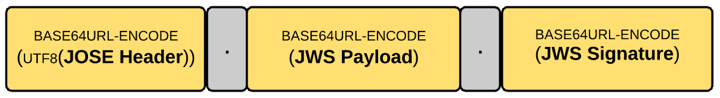
\includegraphics[width=9cm]{Pages/JWS/CompactSerialization.png}
\caption{JWS Compact Serialization}\cite{Compact}
\end{figure}
The dots are representing the concatenation of the components.
In this serialization, the JWS Protected Header is used as the JOSE Header. Therefore, no JWS Unprotected Header will be used.\newline
In contrast to the JWS JSON Serialization, the JWS Compact Serialization provides no syntax for a JWS Unprotected Header and only supports one digital signature/MAC.
In the JWS JSON Serialization there are two related syntaxes: A flattered syntax, to secure content with only one MAC/digital signature and a fully general syntax, for securing with more than one MAC/digital signature \cite{rfc7515}. In this section, only the fully general syntax is treated. 
A JWS in the fully general JWS JSON Serialization ``includes 2 top-level elements: payload and signatures (which is a JSON array), and three sub elements under each entry of the signatures array: protected, header and signature''\cite{Dummies}.
In each entry at least one of the values \texttt{protected} or \texttt{header} must be present to guarantee the texttt{alg} Header Parameter is present \cite{rfc7515}.\newline
An example of this concept can be displayed in Figure 6:\newline 
	\begin{figure}
\centering
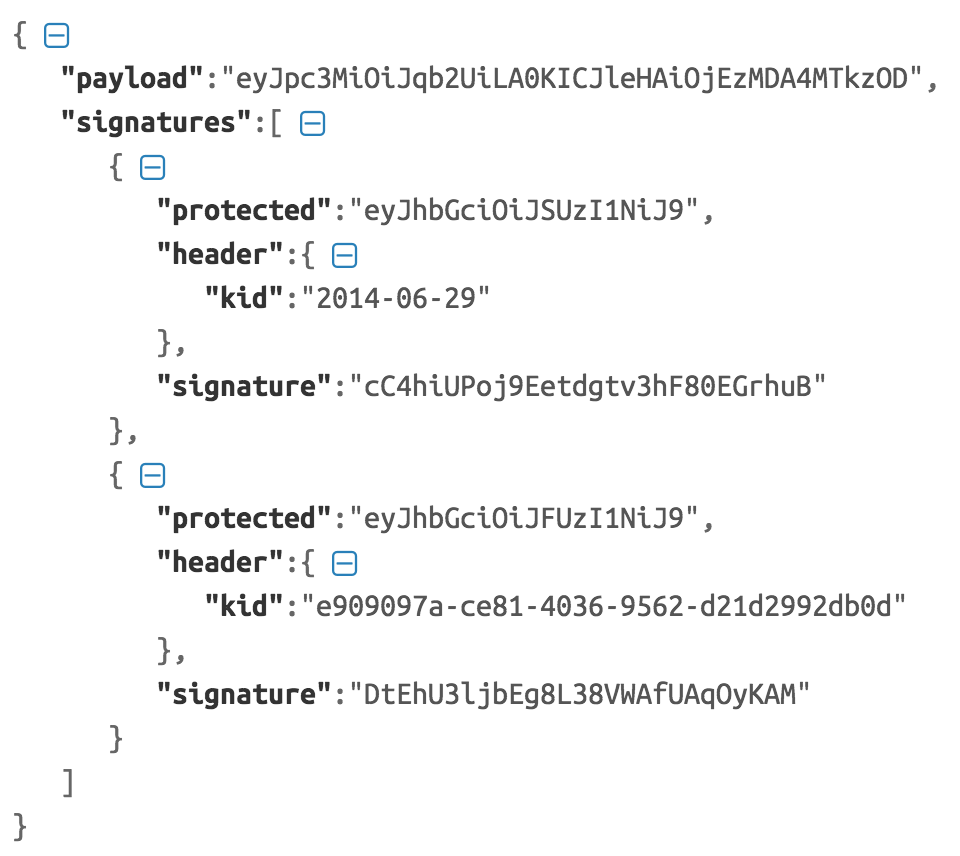
\includegraphics[width=8cm]{Pages/JWS/JSONSerialization.png}
\caption{JWS JSON Serialization} \cite{JSON}
\end{figure}
\subsection{The computation and validation }
For both types of serializations, the computation of a JWS is similar. To create a valid JWS the following steps have to be performed (based on\cite{rfc7515}): 
\begin{enumerate} [leftmargin=1cm,rightmargin=1cm]\itemsep0.2em
\item Generate the desired content, which will be the payload of the JWS.
\item Compute the Base64Url-encoded payload. 
\item ``Create the JOSE Header with the desired set of Header Parameter as a JSON object'' \cite{rfc7515}.
\item Compute the UTF8 representation of the JWS Protected Header and base64url-encode it.
\item Create the signature by using the algorithm, defined in texttt{alg},\newline over the \textbf{JWS Signing Input}, which creation is displayed in Figure 7. 
\begin{figure}
\centering
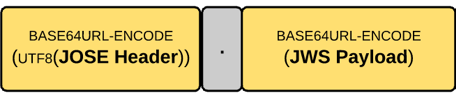
\includegraphics[width=8cm]{Pages/JWS/SigningInput.png}
\caption{JWS Signing Input}\cite{Compact} (Modified)
\end{figure} If \texttt{alg} has the value \texttt{none}, there will be no signature.
\item Compute the encoded signature by base64url-encode the JWS Signature .
\item For the JWS JSON Serialization the steps 3-6 have to be repeated for each MAC/digital signature defined in the JWS JOSE Header.
\item Compute the specific serialization output. For the structure look at the description of JWS Compact Serialization and JWS JSON Serialization.
\end{enumerate} 
After the computation the valid JWS could be placed in the payload of an MQTT message and sent to the intended receiver, where it should be validated.
As the computation of a JWS, the validation of a JWS is again similar for both types of serialization. It is important to note that if there are multiple signatures, like in the fully general JWS JSON Serialization,  it is application-specific how many and which JWS Signatures must be validated successfully \cite{rfc7515}. However, at least one JWS Signature must be validated successfully.
To validate a JWS, the following steps have to be performed (based on\cite{rfc7515}):\newline  
\begin{enumerate} [leftmargin=1cm, rightmargin=1cm] \itemsep0.3em
\item ``Parse the JWS representation to extract the serialized values for the components of the JWS'' \cite{rfc7515}. Look at the specific serialization for the components.
\item Decode the base64url-encoded JWS Protected Header.
\item Verify that the result of step 2 is a UTF8-encoded, valid JSON object.
\item For the JWS Compact Serialisation the JWS Protected header is used as the JOSE Header. For the JWS JSON Serialisation the JWS Protected Header Members and the JWS Unprotected Header Members combined build the JOSE Header.
\item Verify that all fields, which are required to be supported, are understood and can be processed by the implementation.
\item Decode the Base64Url-encoded JWS Payload.
\item Decode the Base64Url-encoded JWS Signature.
\item Validate if the JWS Signing input MACed/digitally signed conformed the JWS Signature.
\item For the JWS JSON Serialisation the steps 4-8 have to be repeated for each MAC/digital signature defined in the JWS JOSE Header.
\item The JWS must be considered invalid if all validations in step 9 failed. (In the case of JWS Compact Serialization it is easy to indicate whether the JWS was validated successfully or not, by the result, whereas in the case of the JWS JSON serialization the result only indicates which validation was successfull and which not.)
\end{enumerate}
How precise a JWS can provide integrity depends on which and how much MACs/digital signatures are being used. If there is no algorithm, integrity cannot be guaranteed. 
\subsection{Input on MQTT packet}
To exemplify the impact of an JWS on a MQTT packet in this section a JWS will be created and appended to the existing MQTT packet from Section 3. \newline As serialization for the JWS the JWS Compact Serialization will be used.
To integrity-protect the message ``integrity can be guaranteed, if you are able to recalculate this part:'' the HMAC with SHA-256 (HS256) will be used along with the key ``e9r3rZrvAqEMkAFRpXP9m8pNAXYAQmT4TcmAdHusePWQBspX98bM\newline xHfkp0bHcNWG''.\newline
Executing the computation steps in chapter 7.4 the following valid JWS is created:\newline eyJhbGciOiJIUzI1NiJ9.aW50ZWdyaXR5IGNhbiBiZSBndWFyYW50ZWVkLC\newline BpZiB5b3UgYXJlIGFibGUgdG8gcmVjYWxjdWxhdGUgdGhpcyBwYXJ0Og.ey\newline JhbGciOiJIUzI1NiJ9.ZWViNGQxYmZhMzA0YWQwNzdiOGM5Y2U1ZWUwN\newline mE5Nzc4MGYwNzZmNQ (line break only for represetational purpose). \newline
To attach the created JWS to the given basic MQTT packet, it must be hexa-decimal encoded resulting in: \newline 65794a68624763694f694a49557a49314e694a392e615735305a576479615852354947\newline4e68626942695a53426e64574679595735305a57566b4c4342705a6942356233556759\newline584a6c494746696247556764473867636d566a5957786a645778686447556764476870\newline6379427759584a304f672e65794a68624763694f694a49557a49314e694a392e5a5756\newline694e475178596d5a684d7a4130595751774e7a64694f474d35593255315a5755774e6\newline d45354e7a63344d4759774e7a5a6d4e51 . \newline Table 4 represents the MQTT packet with the appended JWS is:

\begin{table}[]
\centering
\begin{tabular}{lllllllllllllllll}
45 & 00 & 00 & 8d & 28 & c9 & 40 & 00 &  & 80 & 06 & ec & 47 & c0 & a8 & b2 & 02 \\
c0 & a8 & b2 & 06 & e6 & a4 & 07 & 5b &  & 8b & bf & b9 & 65 & fb & 88 & a4 & e7 \\
50 & 18 & 01 & 00 & 05 & b0 & 00 & 00 &  & 30 & 82 & 1a & 00 & 13 & 2f & 69 & 73 \\
2f & 69 & 74 & 2f & 6f & 66 & 2f & 69 &  & 6e & 74 & 65 & 67 & 72 & 69 & 74 & 79 \\
69 & 6e & 74 & 65 & 67 & 72 & 69 & 74 &  & 79 & 20 & 63 & 61 & 6e & 20 & 62 & 65 \\
20 & 67 & 75 & 61 & 72 & 61 & 6e & 74 &  & 65 & 65 & 64 & 2c & 20 & 69 & 66 & 20 \\
79 & 6f & 75 & 20 & 61 & 72 & 65 & 20 &  & 61 & 62 & 6c & 65 & 20 & 74 & 6f & 20 \\
72 & 65 & 63 & 61 & 6c & 63 & 75 & 6c &  & 61 & 74 & 65 & 20 & 74 & 68 & 69 & 73 \\
20 & 70 & 61 & 72 & 74 & 3a & 65 & 79 &  & 4a & 68 & 62 & 47 & 63 & 69 & 4f & 69 \\
4a & 49 & 55 & 7a & 49 & 31 & 4e & 69 &  & 4a & 39 & 2e & 61 & 57 & 35 & 30 & 5a \\
57 & 64 & 79 & 61 & 58 & 52 & 35 & 49 &  & 47 & 4e & 68 & 62 & 69 & 42 & 69 & 5a \\
53 & 42 & 6e & 64 & 57 & 46 & 79 & 59 &  & 57 & 35 & 30 & 5a & 57 & 56 & 6b & 4c \\
43 & 42 & 70 & 5a & 69 & 42 & 35 & 62 &  & 33 & 55 & 67 & 59 & 58 & 4a & 6c & 49 \\
47 & 46 & 69 & 62 & 47 & 55 & 67 & 64 &  & 47 & 38 & 67 & 63 & 6d & 56 & 6a & 59 \\
57 & 78 & 6a & 64 & 57 & 78 & 68 & 64 &  & 47 & 55 & 67 & 64 & 47 & 68 & 70 & 63 \\
79 & 42 & 77 & 59 & 58 & 4a & 30 & 4f &  & 67 & 2e & 65 & 79 & 4a & 68 & 62 & 47 \\
63 & 69 & 4f & 69 & 4a & 49 & 55 & 7a &  & 49 & 31 & 4e & 69 & 4a & 39 & 2e & 5a \\
57 & 56 & 69 & 4e & 47 & 51 & 78 & 59 &  & 6d & 5a & 68 & 4d & 7a & 41 & 30 & 59 \\
57 & 51 & 77 & 4e & 7a & 64 & 69 & 4f &  & 47 & 4d & 35 & 59 & 32 & 55 & 31 & 5a \\
57 & 55 & 77 & 4e & 6d & 45 & 35 & 4e &  & 7a & 63 & 34 & 4d & 47 & 59 & 77 & 4e \\
7a & 5a & 6d & 4e & 51
\end{tabular}
\caption{Basic packet with valid JWS}
\label{tab:my-table}
\end{table}

\section{Conclusion}

In here our conclusion will be, and so the last real texty chapter.
%\section{sources}

Here we will keep track of all our sorces.

\subsection{Related Work}

\subsection{Other Papers}

\subsection{Pictures}
%\include{Pages/SourcesME}
\newpage
\bibliography{bibtexME}
\bibliographystyle{alpha}
%\section{Appendix A: Contributions}

\begin{longtable}[ht]{|p{0.5\textwidth}|p{0.5\textwidth}|}
\hline
Section & Author \\ \hline \hline
Introduction & Michael Ehrlinger \\ \hline
Related Work: HMAC & Michael Ehrlinger \\ \hline
Related Work: ... & \\ \hline
Related Work: ... & \\ \hline
Related Work: ... & \\ \hline
Message Authentication Codes based on Hash-Functions using HMAC's & Michael Ehrlinger \\ \hline
Digital Signatures using Elliptic Curve Cryptography & Nicolas Salomon \\ \hline
mainbody & Martin Weinhart \\ \hline
mainbody & Vanessa Hermann \\ \hline
Conclusion & ... \\ \hline


\end{longtable}


\end{document}
